Now that the concepts have been presented, let us have a look at how these can be used to create a program. We will take the code from the Hello World, and use a compiler to turn this code into a program that we can then execute. This process is the same for large and small programs.

\subsection{Making the Hello World Program} % (fold)
\label{sub:compiling_code}

\lref{lst:hello-world-c} and \lref{lst:hello-world-pas} show the source code for the Hello World program. To make this into a program you need to:

\begin{enumerate}
  \item Write the code into a text file.
  \item Save the text file to disk.
  \item Compile it.
\end{enumerate}

Step 1 and 2 can be accomplished with any text editor, but the best ones to use highlight your code. Each programming language has rules that determine how its code must be formatted. This is known as the language's \textbf{syntax}. You can get text editors that understand these rules, and highlight your code as you type. This is called \textbf{syntax highlighting}. This highlighting can help you identify any little mistakes you make. \fref{fig:linux-editors} shows the Hello World code in gedit in Linux. \fref{fig:mac-editors} shows the code in TextMate on Mac OS. \fref{fig:windows-editors} shows the code in Notepad++ in Windows.

\begin{figure}[h]
   \centering
   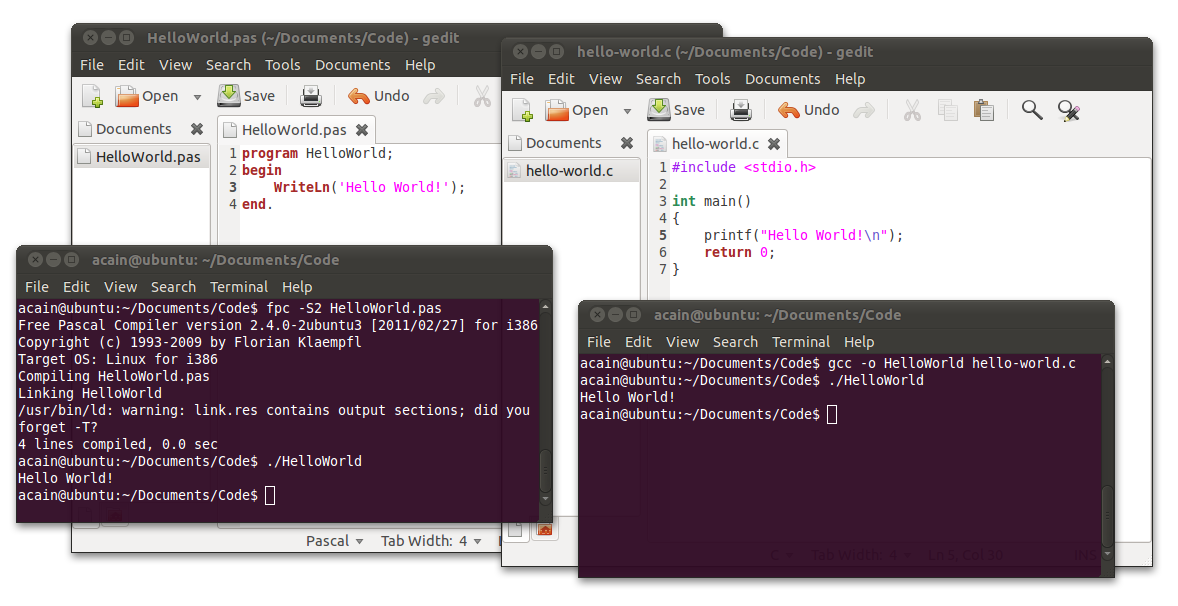
\includegraphics[width=\textwidth]{./topics/programs-and-compilers/images/LinuxEditors} 
   \caption{Editing and Compiling C and Pascal code in Linux}
   \label{fig:linux-editors}
\end{figure}

\begin{figure}[h]
   \centering
   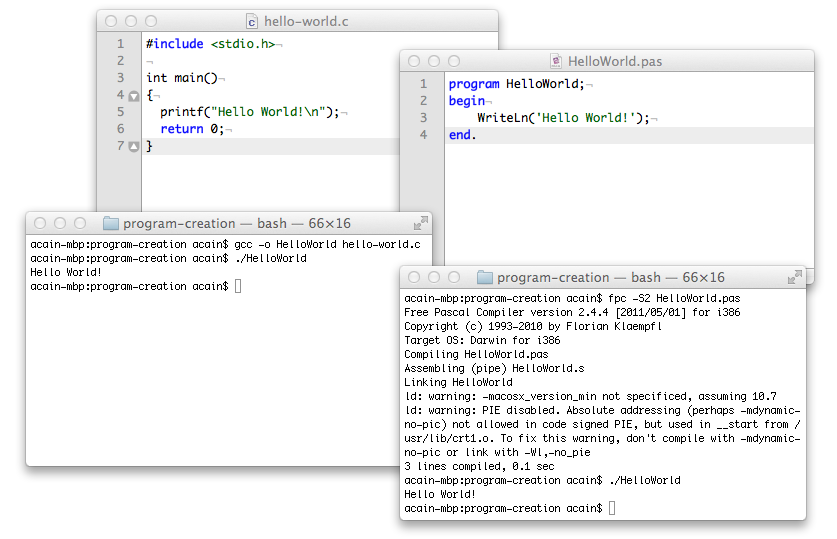
\includegraphics[width=\textwidth]{./topics/programs-and-compilers/images/MacEditors} 
   \caption{Editing and Compiling C and Pascal code in Mac OS}
   \label{fig:mac-editors}
\end{figure}

\begin{figure}[h]
   \centering
   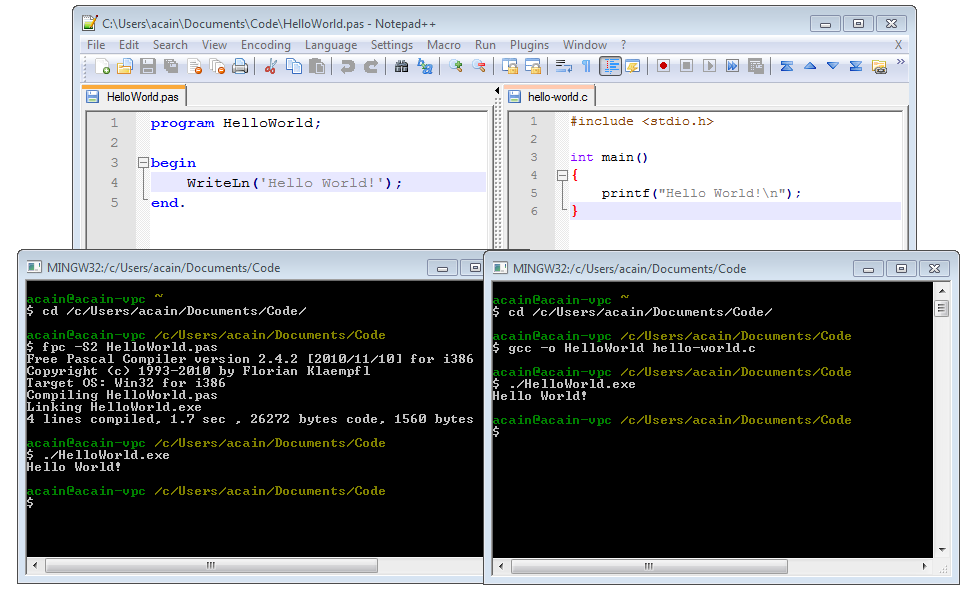
\includegraphics[width=\textwidth]{./topics/programs-and-compilers/images/WindowsEditors} 
   \caption{Editing and Compiling C and Pascal code in Windows}
   \label{fig:windows-editors}
\end{figure}


\mynote{
\begin{itemize}
  \item Syntax highlighting editors include:
  \begin{itemize}
    \item \textbf{gedit} on Linux.
    \item \textbf{TextMate} or \textbf{TextWrangler} on MacOS.
    \item \textbf{Notepad++} or \textbf{Crimson Editor} on Windows.
  \end{itemize}
  \item Take care when you type the code in, even one character out of place may mean the compiler fails to compile your code.
\end{itemize}
}

\clearpage
\subsubsection{Running the Compiler} % (fold)
\label{ssub:running_the_compiler}

Once you have saved the code to file it is time to compile your program. For this you are going to need to open a \nameref{sub:terminal}, and change into the directory where you saved the source code file. Once you are in this directory it is time to run the compiler.

When you run the compiler you need to give it two kinds of information: options, and the name of the file to compile. The compiler will read the code in the file you give it, and convert this to machine code as shown in \sref{sub:source_code_and_the_compiler} \nameref{sub:source_code_and_the_compiler}. The exact command you use depends on the compiler you are using.

\csection{
In C the compiler we will be using is called \textbf{gcc}, which stands for the \textbf{GNU C Compiler}. The command you need to run in the Terminal is shown in Listing \ref{lst:compile-hello-world-c}. The \emph{-o name} option tells gcc the name of the program file to create. In our example this will compile the code in \emph{hello-world.c} and save the machine code into a program called \emph{HelloWorld}.

\bashcode{lst:compile-hello-world-c}{Compiling C code.}{code/c/program-creation/compile-hello-world.sh}
}

\passection{
In Pascal the compiler we will be using is called \textbf{fpc}, which stands for the \textbf{Free Pascal Compiler}. The command you need to run in the Terminal is shown in Listing \ref{lst:compile-hello-world-pas}. The \emph{-S2} option is used to tell fpc to compile using the latest `Free Pascal' version of the language. In our example this will compile the code in \emph{HelloWorld.pas} and save the machine code into a program called \emph{HelloWorld}, which it gets from the name of the Pascal file.

\bashcode{lst:compile-hello-world-pas}{Compiling Pascal code.}{code/pascal/program-creation/compile-hello-world.sh}
}

Once you get the program to compile you can run it! This will load your program into memory, and start its steps running. The HelloWorld program will output the text `\texttt{Hello World!}' to the Terminal. To run the program you need to use its name. The command you need to enter is shown in \lref{lst:run-hello-world}, and in \fref{fig:run-helloworld}. The \texttt{./} before the file tells Bash to look in the current directory for the program.

\bashcode{lst:run-hello-world}{Bash command to run HelloWorld}{topics/programs-and-compilers/run-hello-world.sh}

\begin{figure}[h]
   \centering
   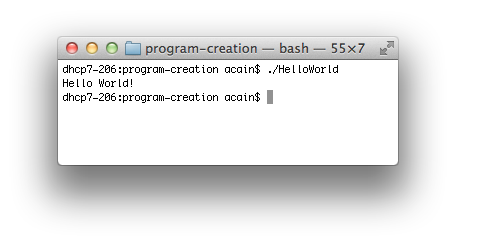
\includegraphics[width=0.7\textwidth]{./topics/programs-and-compilers/images/HelloWorld} 
   \caption[Hello World Terminal]{Hello World run from the Terminal}
   \label{fig:run-helloworld}
\end{figure}

% subsubsection running_the_compiler (end)

\subsubsection{When things do not work} % (fold)
\label{ssub:when_things_do_not_work}

Compilers are very specific about the code you give it. If the source code you try to compile does not follow all of the rules of the language then the compiler will fail, and end with an error message. These errors, called \textbf{syntax errors}, could be as small as missing a semicolon (;), or misspelling a name. To get your program to compile you will need to correct any syntax errors the compiler finds in your code.

\begin{figure}[h]
   \centering
   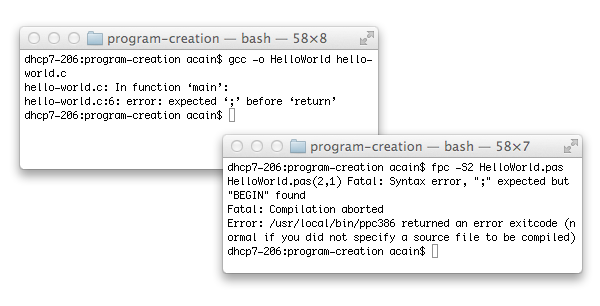
\includegraphics[width=0.8\textwidth]{./topics/programs-and-compilers/images/SyntaxErrors} 
   \caption{These Terminals show some syntax errors from programs that are missing a single semicolon (;)}
   \label{fig:syntax-errors}
\end{figure}

\fref{fig:syntax-errors} shows an example output caused by removing a single semicolon from the Hello World program's code. The numbers in the error messages give you an idea of where the compiler got to when it encountered the error. So the text \texttt{hello-world.c:6:} output from the C compiler indicates that the compiler got to line 6 before it encountered the error. The text \texttt{HelloWorld.pas(2,1)} output from the Pascal compiler indicates that it got up to line 2 character 1 before it encountered the error.

When the compiler encounters these issues it does not create the executable program. You need to learn to use these error messages to help you locate errors in your code, so that you can fix them, and then run the compiler again to generate your program.

\mynote{
\begin{itemize}
  \item Syntax errors are very common. Do not worry when this occurs to you.
  \item Always start with the first error. The compiler will try to continue compiling your code after it finds an error. This can mean that later errors do not really exist, once you fix the earlier ones.
  \item Unfortunately compiler error messages are not always very clear on what the cause of the error is. You need to learn how to read and understand these messages.
  \item To get good at programming requires lots of practice.
\end{itemize}
}

% subsubsection when_things_do_not_work (end)



% section the_compiler (end)
